% Created 2023-02-15 mer. 14:17
% Intended LaTeX compiler: pdflatex
\documentclass[presentation]{beamer}
\usepackage[utf8]{inputenc}
\usepackage[T1]{fontenc}
\usepackage[french]{babel}
\usepackage[labelformat=empty]{caption}
\usepackage{verbatim}
\definecolor{purple_wada}{RGB}{128,71,189} %   #8047bdff
\definecolor{links}{HTML}{2A1B81}
\useoutertheme{infolines}
%
% Beamer options
%
\setbeamertemplate{caption}{\raggedright\insertcaption\par}
\setbeamercovered{transparent}
\setbeamertemplate{section in toc}[sections numbered]
\setbeamertemplate{subsection in toc}[square]
\setbeamertemplate{navigation symbols}{}
\setbeamercolor{section in head/foot}{bg=purple_wada, fg=white}
\setbeamercolor{subsection in head/foot}{bg=white, fg=purple_wada}
\setbeamercolor{title in head/foot}{fg=purple_wada,bg=white}
\setbeamercolor{author in head/foot}{fg=white,bg=purple_wada}
\setbeamercolor{date in head/foot}{fg=white,bg=purple_wada}
\setbeamercolor{frametitle}{fg=purple_wada,bg=white}
\setbeamercolor{block title}{fg=purple_wada,bg=white}
%
% Adding frame at each section
%
\AtBeginSubsection[]
{
\begin{frame}
\frametitle{Sommaire}
\tableofcontents[currentsection,currentsubsection]
\end{frame}
}
\hypersetup{
colorlinks,
allcolors=.,
urlcolor=blue,
}
\usetheme{default}
\author{Doc. Malik Koné}
\date{04/02/2023}
\title{Transactions on blockchains}
\hypersetup{
 pdfauthor={Doc. Malik Koné},
 pdftitle={Transactions on blockchains},
 pdfkeywords={},
 pdfsubject={},
 pdfcreator={Emacs 28.2 (Org mode 9.4.6)}, 
 pdflang={French}}
\begin{document}

{
  \usebackgroundtemplate{
\includegraphics[height=\paperheight]{./page_de_garde_wadaci_j4.png}}
  \frame[plain]{
  }
}

\section{Tutoriel 1: Communiquer avec un noeud Cardano}
\label{sec:org5cf7404}
\subsection{Mise en place}
\label{sec:orgace94cc}
\begin{frame}[label={sec:orgff8e439}]{Créer un compte sur la Plateforme}
      \begin{center}
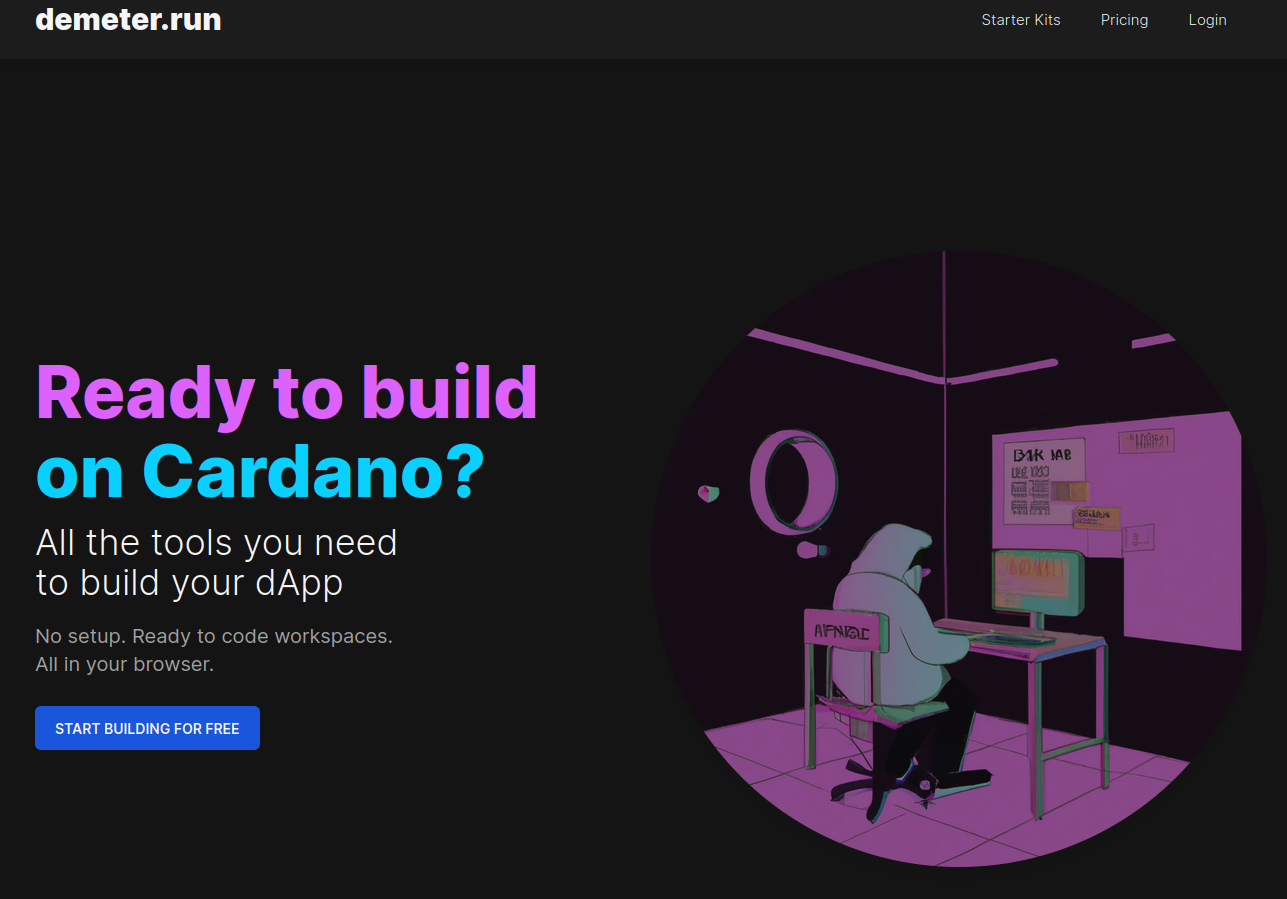
\includegraphics[height=.7\textheight]{Images/demeter_run.png}
\end{center}
Liens vers la plateforme -> \href{http://demeter.rum}{demeter.run}
\end{frame}

\subsection{Tutoriel}
\label{sec:org644d296}
\begin{frame}[label={sec:org7c61081}]{Communiquer avec un noeud Cardano}
Lien github -> \href{https://github.com/txpipe/cardano-cli-starter-kit}{Cardano-cli.git}
\begin{center}
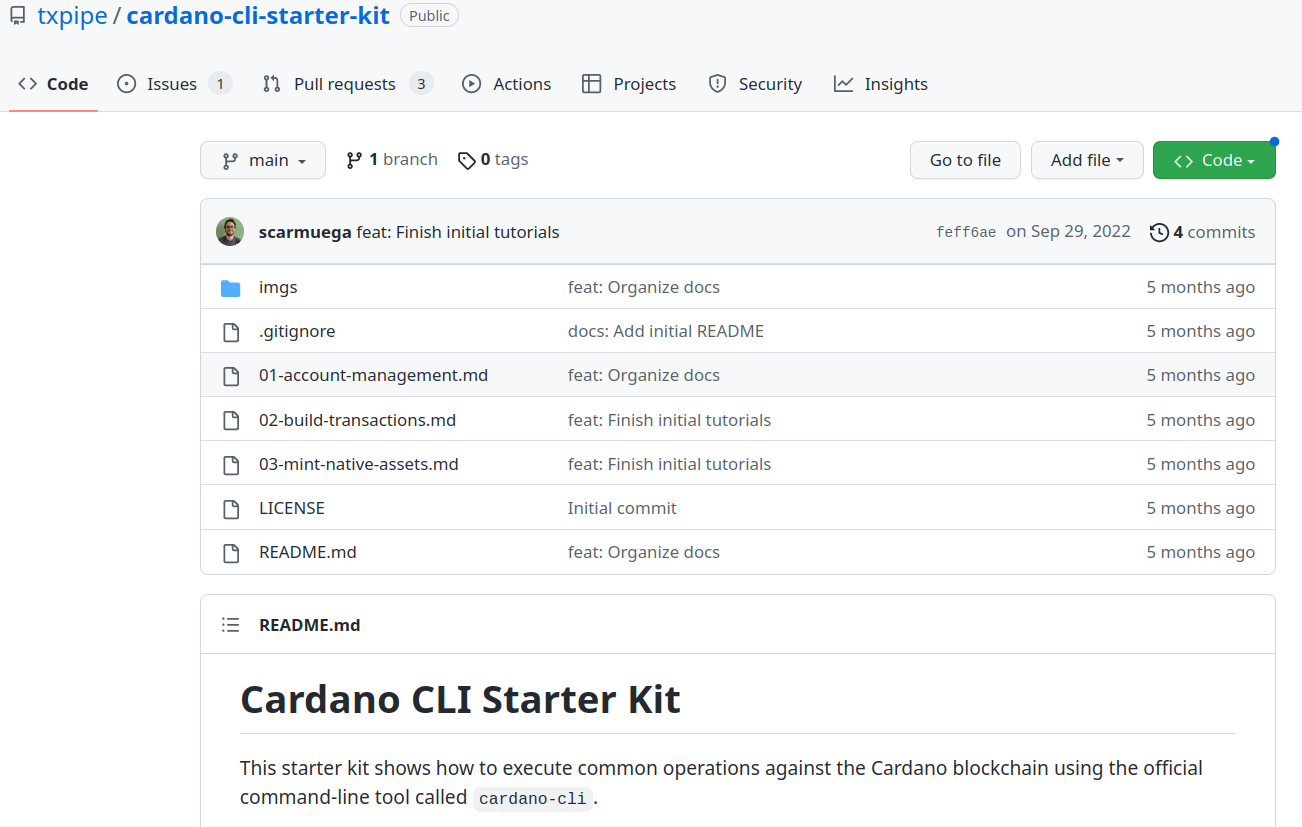
\includegraphics[height=.7\textheight]{Images/tuto_cardano_cli.png}
\end{center}
\end{frame}

\section{Script Plutus : Une introduction à Haskell}
\label{sec:org8bdf76f}
\subsection{Enchère à l'anglaise}
\label{sec:org392ca42}
\begin{frame}[label={sec:org40483a6}]{Alice propose une enchère (1/4)}
\begin{center}

\includegraphics[height=.5\textheight]{Images/enchere_01.png}
\end{center}
\begin{columns}
\begin{column}{0.3\columnwidth}
\begin{block}{Alice fournit}
\begin{itemize}
\item le NFT
\item un datum (avec l'offre minimal)
\end{itemize}
\end{block}
\end{column}
\begin{column}{0.7\columnwidth}
\begin{block}{Le smart-contract contient}
\begin{itemize}
\item conditions de validité de l'offre (on-chain)
\item logique pour fin d'enchère (off-chain)
\end{itemize}
\end{block}
\end{column}
\end{columns}
\end{frame}
\begin{frame}[label={sec:org3eaac3c}]{Bob fait une offre, nouvelle transaction (2/4)}
\begin{center}
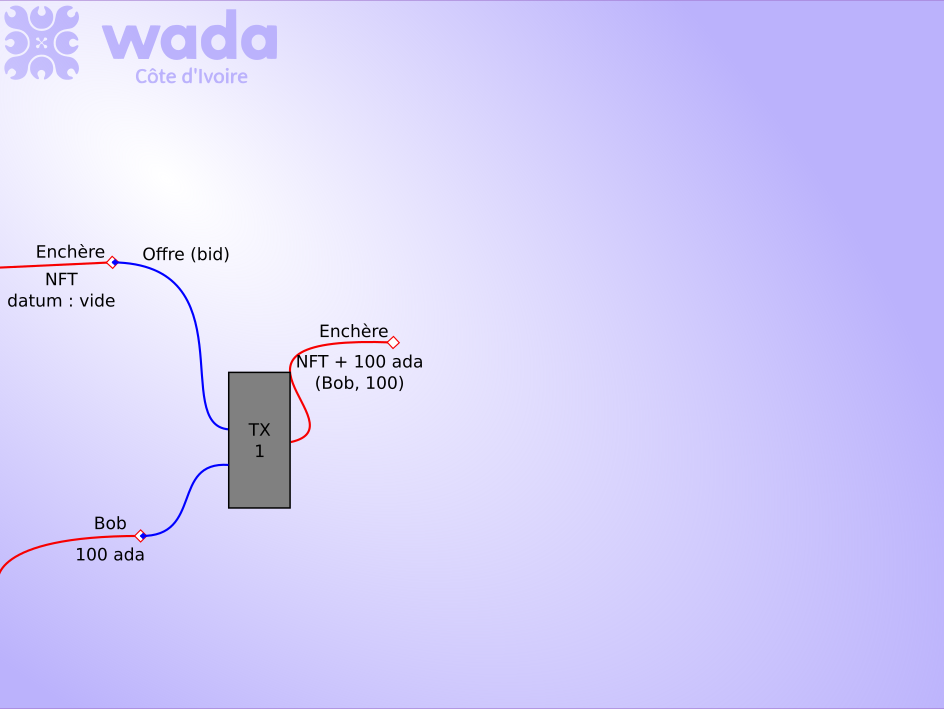
\includegraphics[height=.55\textheight]{Images/enchere_02.png}
\end{center}

\begin{columns}
\begin{column}{0.3\columnwidth}
\begin{block}{En entrée}
\begin{itemize}
\item UTxO d'Alice
\item UTxO de Bob
\end{itemize}
\end{block}
\end{column}
\begin{column}{0.7\columnwidth}
\begin{block}{En sortie}
\begin{itemize}
\item adresse du script -> NFT, datum (Bob, 100)
\end{itemize}
\end{block}
\end{column}
\end{columns}
\end{frame}

\begin{frame}[label={sec:orga791965}]{Charlie sur-offre (3/4)}
\begin{center}
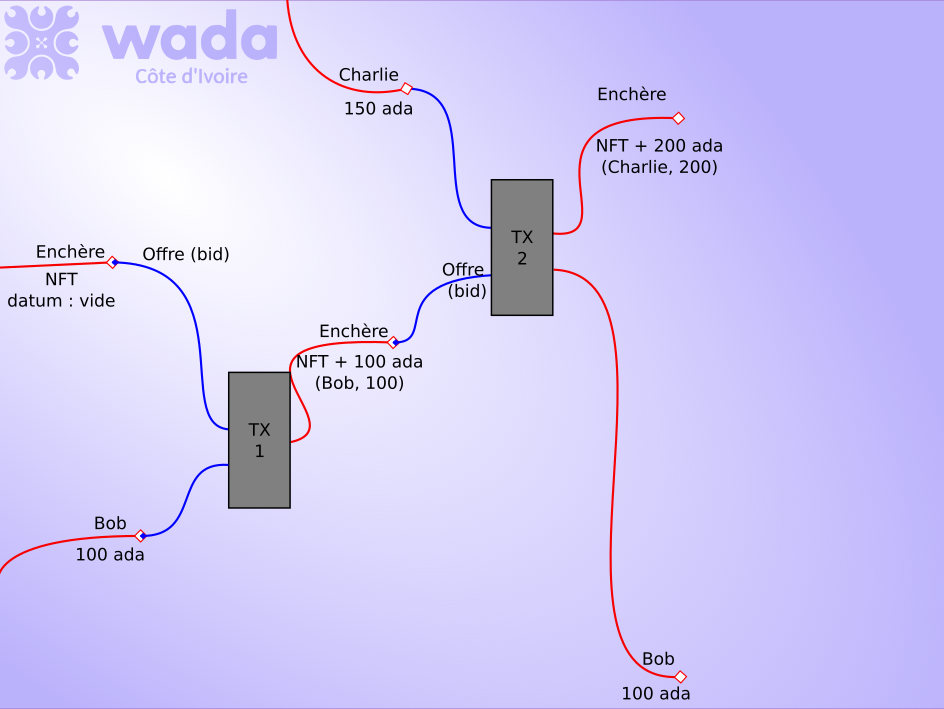
\includegraphics[height=.55\textheight]{Images/enchere_03.png}
\end{center}

\begin{columns}
\begin{column}{0.3\columnwidth}
\begin{block}{En entrée}
\begin{itemize}
\item UTxO du script
\item UTxO de Charlie
\end{itemize}
\end{block}
\end{column}
\begin{column}{0.7\columnwidth}
\begin{block}{En sortie}
\begin{itemize}
\item adresse du script -> NFT, datum (Charlie, 150)
\item adresse de Bob -> 100
\end{itemize}
\end{block}
\end{column}
\end{columns}
\end{frame}

\begin{frame}[label={sec:org39e36d5}]{Fin de l'enchère (4/4)}
      \begin{center}
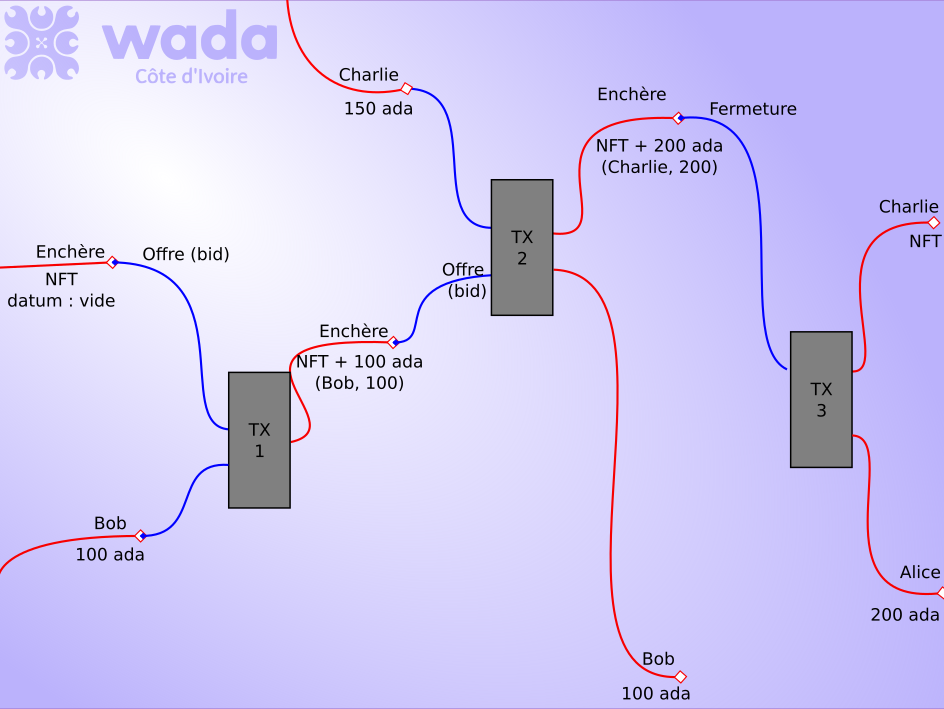
\includegraphics[height=.55\textheight]{Images/enchere_04.png}
\end{center}
Après un certain temps décidé par Alice ou le script
\begin{columns}
\begin{column}{0.3\columnwidth}
\begin{block}{En entrée}
\begin{itemize}
\item UTx0 du script
\end{itemize}
\end{block}
\end{column}
\begin{column}{0.7\columnwidth}
\begin{block}{En sortie}
\begin{itemize}
\item adresse Charlie -> le NFT
\item adresse Alice -> le montant
\end{itemize}
\end{block}
\end{column}
\end{columns}
\end{frame}
\subsection{Code d'un smart contract}
\label{sec:org96aa904}
\begin{frame}[label={sec:orgfbad046}]{Code d'un smart contract}
\begin{center}
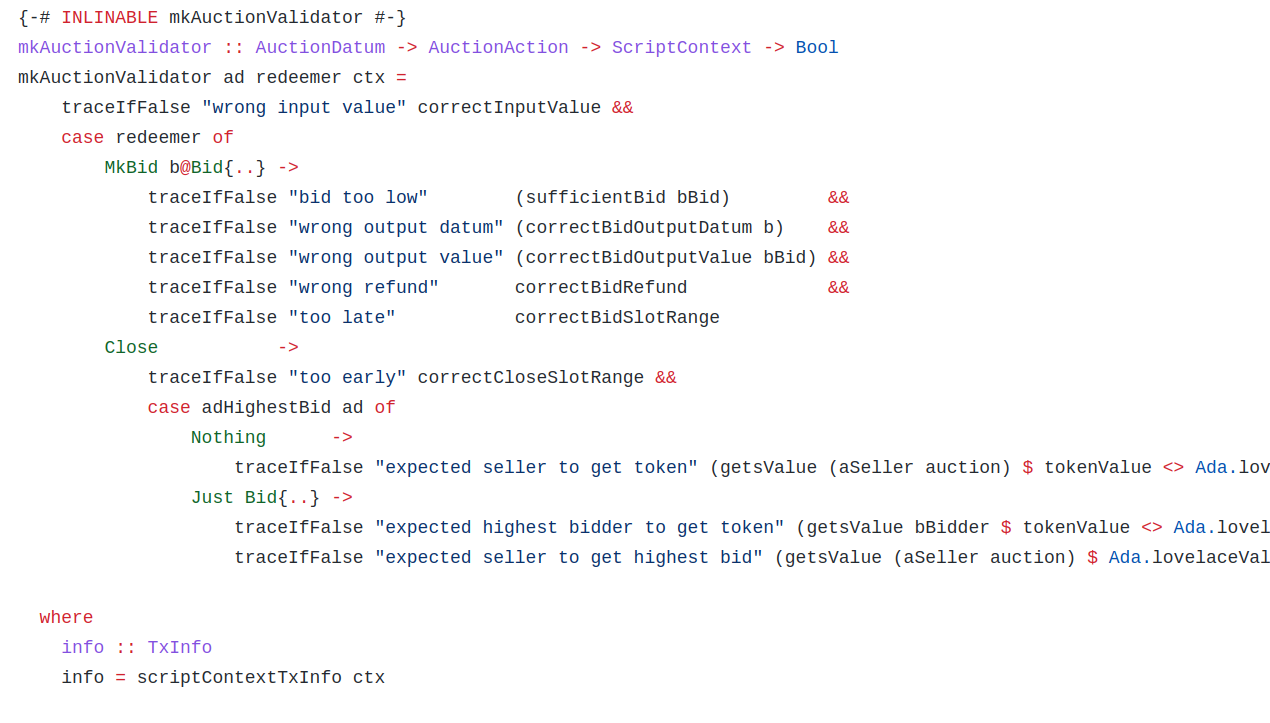
\includegraphics[height=.55\textheight]{Images/smart-contract-plutus.png}
\end{center}

Voir Github du \href{https://github.com/input-output-hk/plutus-pioneer-program/blob/main/code/week01/src/Week01/EnglishAuction.hs}{programme pionniers de plutus} pionneer
\end{frame}
\begin{frame}[label={sec:org7b622f1}]{Survol du code}
\begin{columns}
\begin{column}{0.5\columnwidth}
\begin{block}{}
\begin{block}{on chain}
le code Haskell qui compilé, pour
\begin{itemize}
\item UPLC : plutus-core
\end{itemize}
\end{block}
\begin{block}{off chain}
Le code qui ne réside pas sur la blockchain.
\begin{itemize}
\item Sert à construire une transaction valide
\item Se trouve généralement dans le portefeuille
\end{itemize}
\end{block}
\end{block}
\end{column}
\end{columns}
\end{frame}
\begin{frame}[label={sec:org28c84cf}]{}
\begin{block}{Différentes parties du code}
\begin{itemize}
\item data
\item script
\item compilation
\item validation
\item mockup code for playground
\end{itemize}
\end{block}
\end{frame}

\subsection{Compilation  : plutus template}
\label{sec:orgf83eb87}
\begin{frame}[label={sec:orga8277a0},fragile]{Compilation  : plutus template}
 Partie du code qui compile en UPLC
\begin{verbatim}
typedAuctionValidator :: Scripts.TypedValidator Auctioning
typedAuctionValidator = Scripts.mkTypedValidator @Auctioning
    $$(PlutusTx.compile [|| mkAuctionValidator ||])
    $$(PlutusTx.compile [|| wrap ||])
  where
    wrap = Scripts.wrapValidator @AuctionDatum @AuctionAction

\end{verbatim}
\end{frame}

\section{Tutoriel 2 : Comment compiler un script plutus et l'activer}
\label{sec:org7ddf95e}
\subsection{Tutoriel}
\label{sec:org15c2fb8}
\begin{frame}[label={sec:org1f886f8}]{Comment compiler un script plutus et l'activer}
      \begin{center}
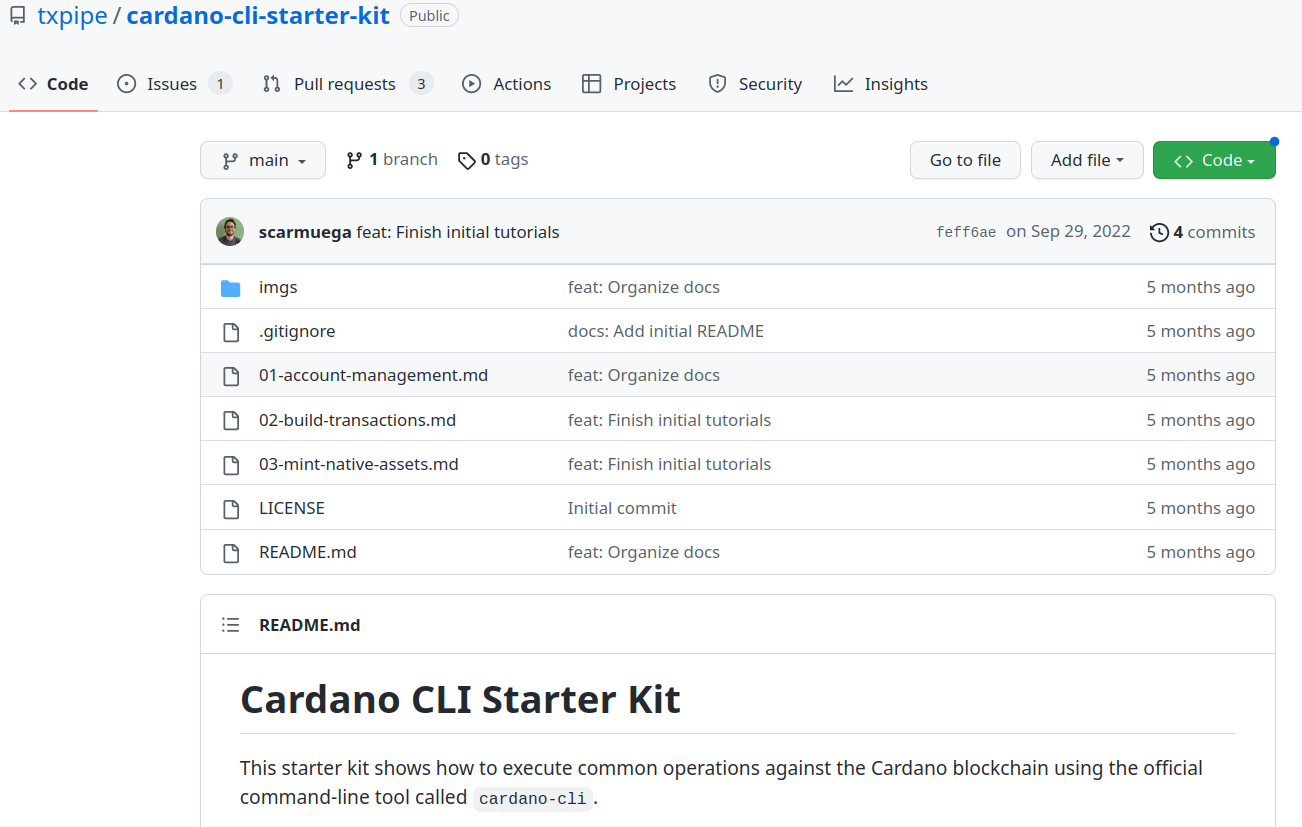
\includegraphics[height=.7\textheight]{Images/tuto_cardano_cli.png}
\end{center}
Lien github -> \href{https://github.com/txpipe/plutus-starter-kit}{plutus-start-kit.git}
\end{frame}
\section{Références}
\label{sec:orgb5b99b7}
\subsection{Références}
\label{sec:org141f723}
\begin{frame}[label={sec:orge80a8b7}]{Liens des références}
\begin{block}{IOG Academy}
Lien -> \href{https://www.youtube.com/@iogacademy/playlists}{Vidéos et ressources devenir expert en Marlow, Plutus et Haskell}
\end{block}

\begin{block}{Plutus pioneer programm}
Lien -> \href{https://www.youtube.com/@iogacademy/playlists?view=50\&sort=dd\&shelf\_id=3}{Plutus pioneer program} Lars Brünjes
\end{block}
\begin{block}{Tutoriels Demeters}
\begin{itemize}
\item \href{https://github.com/orgs/txpipe/repositories}{Github de txpipe}
\end{itemize}
\begin{block}{D'autre tutos}
\begin{itemize}
\item \url{https://github.com/iburzynski/emurgo-plutus-starter}
\item \url{https://github.com/input-output-hk/Alonzo-testnet}
\end{itemize}
\end{block}
\end{block}
\end{frame}
\end{document}